\section{Wykorzystane technologie}
Do stworzenia aplikacji wykorzystano wiele technologii oraz narzędzi deweloperskich opisanych w poniższych podrozdziałach.

\subsection{Java 8}
Aplikacja w całości została napisana w języku Java.
Java jest językiem programowania ogólnego przeznaczenia, zorientowanym obiektowo. Posiada obsługę wyjątków oraz naturalne wsparcie dla wielowątkowości, pozwala na szybkie tworzenie wysokopoziomowych aplikacji. Aplikacje napisane w języku Java kompilowane są do kodu bajtowego, który uruchamiany jest przez wirtualną maszynę Javy (JVM), niezależnie od architektury urządzenia.

Dzięki wieloplatformowości stworzona aplikacja może być uruchamiana na każdym systmie operacyjnym z wirtualną maszyną Javy.

W projekcie aplikacji wykorzystano język Java w wersji 8. 
Pozwoliło to na użycie w projekcie takich elementów języka, jak: wyrażenia lambda i interfejsy funkcyjne (skracające zapis i zwiększające czytelność kodu) oraz strumieni (stream API) - do szybkiego i przejrzystego przekształcania i filtracji danych.

\subsection{JavaFX}
JavaFX jest platformą do tworzenia aplikacji desktopowych (okienkowych) pisanych w języku Java.
Od wersji 8 JavaFX została właczona do platformy Java Standard Edition.
Jest to nowsze, obecnie zalecane przez firmę {\it Oracle} rozwiązanie do tworzenia aplikacji okienkowych. Nie zaleca się natomiast korzystania z bibliotek {\it AWT} lub {\it Swing} \ref{javafx-replacing-swing}.

Do zbudowania widoków aplikacji wykorzystano specjalny format plików FXML, w którym to JavaFX przechowuje informację o właściwościach komponentów interfejsu użytkownika oraz o ich wzajemnych relacjach.

\subsection{Spring}
\subsubsection{Spring Framework}
Spring jest frameworkiem, który umożliwia w aplikacjach Javy zastosowanie wzorca architektonicznego odwrócenia sterowania (ang. {\it Inversion of Control}), a w szczególności wstrzykiwania zależności (ang. {\it Dependency Injection}). Pozwala to uniknąć występowania bezpośrednich zależności pomiędzy komponentami oraz umożliwia automatyczne dostarczanie i zarządzanie cyklem życia komponentów aplikacji.

W zaprojektowanej aplikacji Spring jest wykorzystywany m.in. do automatycznego dostarczania współdzielonych danych o parametrach symulacji oraz do zarządzania cyklem życia kontrolerów i widoków z biblioteki JavaFX.

\subsubsection{Spring Boot}
Spring Boot jest rozwiązaniem przyspieszającym proces konfiguracji, tworzenia oraz uruchamiania aplikacji opartych na Spring Framework.
Jest to zestaw wstępnie skonfigurowanych komponentów, dzięki którym jeszcze łatwiejsze staje się dołączenie nowych bibliotek zewnętrznych do aplikacj. Celem jest pozbycie się zbędnych konfiguracji w plikach XML a zastąpienie ich domyślnym zestawem konfiguratorów, gdyż większość komponentów w aplikacji zazwyczaj konfigurowana jest w typowy, powtarzalny sposób \ref{docs-springboot}.

Spring Boot dostarcza do aplikacji symulacyjnej wiele zależności do bibliotek (np. logback) oraz dostarcza konfigurację dla systemu budowania Maven.
\subsubsection{Spring Boot JavaFx Support}
{\it Spring Boot JavaFx Support} jest niewielką biblioteką umożliwiającą użycie Spring Boot w jednym projekcie w połączeniu z JavaFx.

\subsection{jUnit i TDD}
jUnit jest frameworkiem do wykonywania testów jednostkowych dla aplikacji napisanych w Javie.

W projekcie zastosowano podejście {\it Test-driven development} dla procesu rozwoju oprogramowania. Dotyczy to rozwoju logiki silnika planowania tras dla algorytmu A* i WHCA*. Algorytm WHCA* jest na tyle złożony, że zdecydowano się najpierw napisać szczególne przypadki testowe, które określały jakie dane wyjściowe są oczekiwane przy zadanych danych wejśiowych. Dopiero po takim pokryciu testami przystąpiono do implementacji algorytmu. Warunkiem poprawności zaimplementowanego algorytmu było, aby wszystkie testy jednostkowe wykonały się prawidłowo. Na tym właśnie podejściu opiera się proces TDD (ang. {\it Test-driven development}), który jest wspierany przez framework jUnit.

\subsection{Maven}
{\it Apache Maven} jest narzędziem do automatyzacji procesu budowania aplikacji napisanych w języku Java.
Przy pierwszym wykorzystaniu zadeklarowanych bibliotek Maven automatycznie pobiera biblioteki ze swojego repozytorium i rozwiązuje wszystkie brakujące zależności do nich. Użytkownik zatem nie musi martwić się o brakujące biblioteki i o manualne dołaczanie ich do projektu.

Narzędzie to zostało użyte w aplikacji do kompilacji ze źródeł oraz uruchamiania. Domyślna konfiguracja procesu budowania dla Maven została zapewniona przez Spring Boot. Uruchomienie aplikacji z kodów źródłowych następuje po wykonaniu w systemie polecenia: $mvn spring-boot:run$.
Do kompilacji i uruchomienia całej aplikacji wystarczy zatem, aby w systemie operacyjnym było zainstalowane środowisko Java JDK oraz {\it Apache Maven}.

\subsection{IntelliJ IDEA}
IntelliJ IDEA jest zintegrowanym środowiskiem deweloperskim przeznaczonym głównie do rozwoju aplikacji w języku Java.
Podczas opracowywania aplikacji korzystano z wersji IntelliJ IDEA Ultimate 2017.2.6, z licencji studenckiej. Zrzut ekranu podczas pracy ze środowiskiem zaprezentowano na rysunku \label{fig:app-tech-intellij}.
Środowisko to zapewnia integrację ze wszystkimi technologiami wymienionymi w tym podrozdziale.
Aplikacja była rozwijana i testowana na systemach operacyjnych z jądrem Linux (Arch Linux oraz Debian 9), jednak wszystkie wymienione narzędzia oraz technologie są wieloplatformowe i z powodzeniem mogą być uruchomione na innych systemach opearcyjnych (Windows, macOS)

\begin{figure}
	\centering
	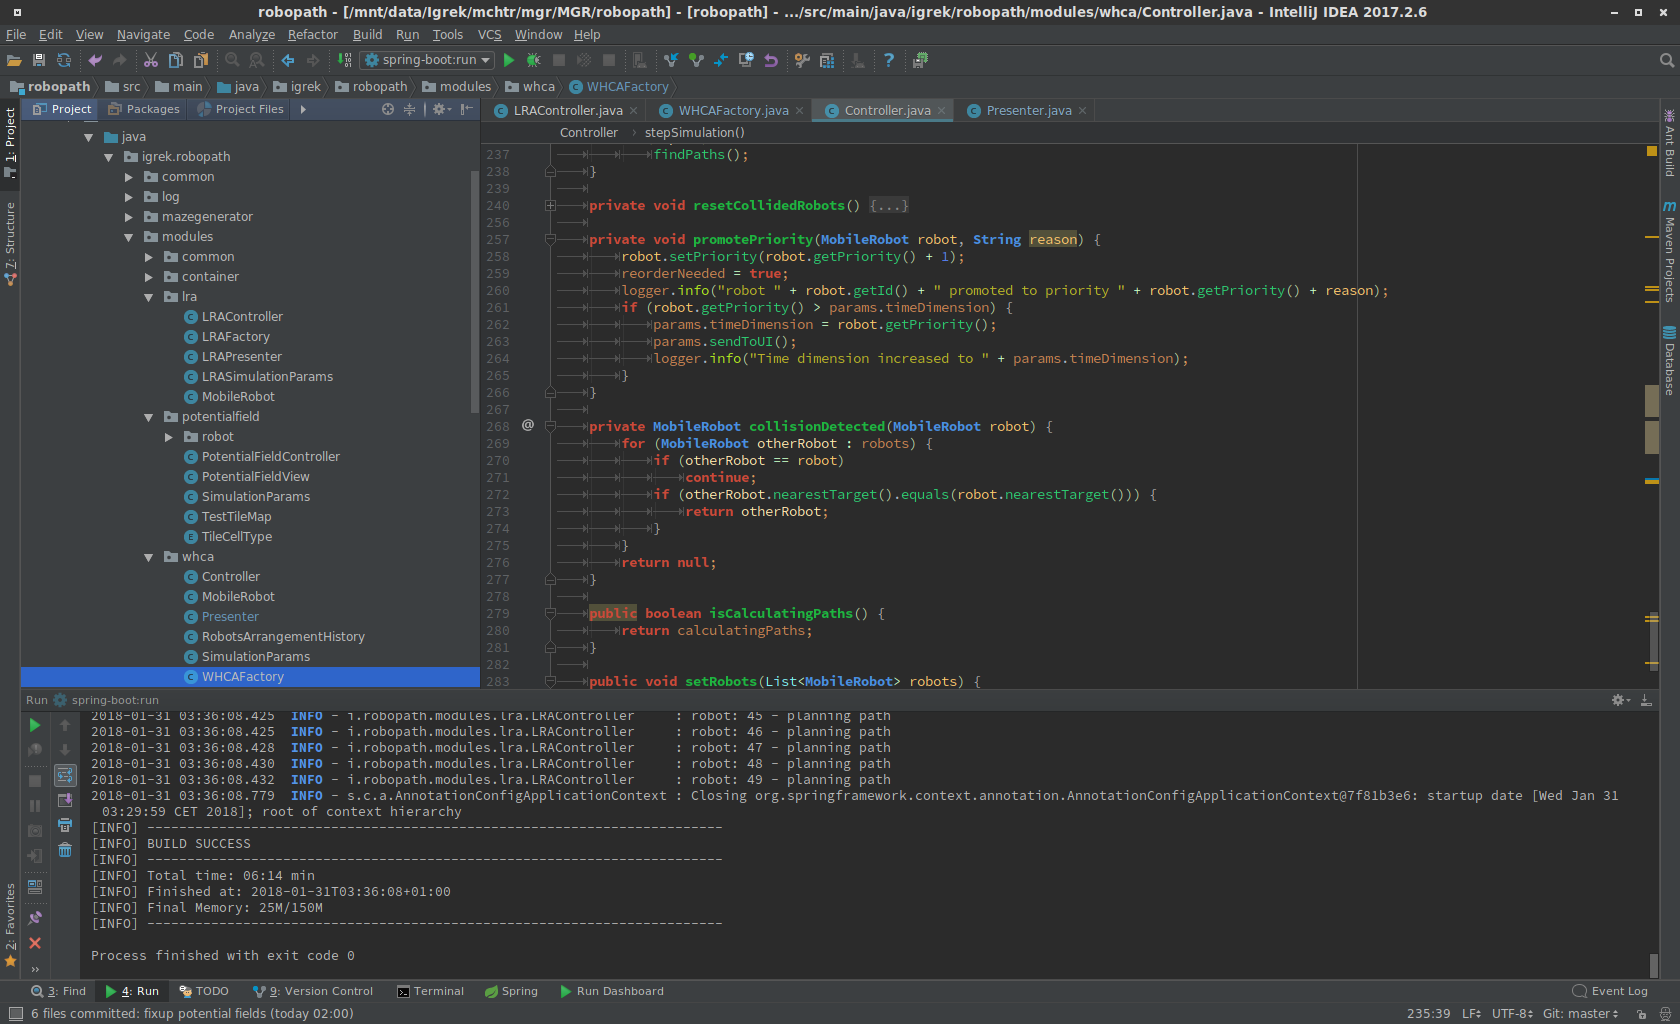
\includegraphics[width=0.9\columnwidth]{img/robopath/intellij}
	\caption{Zrzut ekranu środowiska deweloperskiego Intellij IDEA Ultimate}
	\label{fig:app-tech-intellij}
\end{figure}

\subsection{Pozostałe narzędzia i biblioteki}
\subsubsection{Guava}
Guava jest biblioteką rozwijaną przez Google dostarczającą do Javy m.in. nowe typy kolekcji (struktur danych). W rozwijanej aplikacji wykorzystano ją m.in. do przetwarzania łańcuchów tekstowych.
\subsubsection{git}
Do śledzenia i zapisywania zmian wykorzystano w projekcie system kontroli wersji {\it git}.
Kody źródłowe aplikacji są ogólnie dostępne w repozytorium git na portalu GitHub:
$TODO$ adres
\subsubsection{Logback}
Do zapisu dziennika zdarzeń w aplikacji została wykorzystana biblioteka {\it Logback}, która jest domyślnie dostarczana do aplikacji i skonfigurowana dzięki {\it Spring Boot}.


\section{Struktura aplikacji}
$TODO$ lista beanów / serwisów, struktura widok, prezenter, kontroler; osobny wątek w tle do obliczeń + synchronizacja, wątek UI - zapewnienie REal-time, prawie MVP + MVC


\section{Screeny}
$TODO$ screeny

\section{featurey}
ustawianie random seeda
ponowne wykonanie symulacji - te same warunki
przełaczanie między metodami na zakładkach ?
wykonanie symulacji w pojedynczych krokach
resizable window - responsive
heuristic cache
działania na wektorach, immutable vector

\section{Ograniczenia}
$TODO$ nałożone uproszczenia: ruch skośny trwa tyle samo, czas dyskretny, brak czasu na obrót

$TODO$ publikacja na GitHub, licencja MIT, filmiki na YT